\iffalse
\title{Assignment Gate}
\author{RONGALI CHARAN}
\section{me}
\chapter{2007}
\fi

\item In a machine shop, pins of 15 mm diameter are produced at a rate of 1000 per month and the same is consumed at a rate of 500 per month. The production and consumption continue simultaneously till the maximum inventory is reached. Then inventory is allowed to reduce to zero due to consumption. The lot size of production is 1000. If backlog is not allowed, the maximum inventory level is  
\begin{enumerate}
    \item 400
    \item 500
    \item 600
    \item 700
\end{enumerate}

\item The net requirements of an item over 5 consecutive weeks are 50-0-15-20-20. The inventory carrying cost and ordering cost are Rs. 1 per item per week and Rs. 100 per order respectively. Starting inventory is zero. Use ``Least Unit Cost Technique'' for developing the plan. The cost of the plan (in Rs.) is  
\begin{enumerate}
    \item 200
    \item 250
    \item 255
    \item 260
\end{enumerate}

\textbf{Common Data Questions}

\subsection{Common Data for Questions 71, 72, 73:}  
A gear set has a pinion with 20 teeth and a gear with 40 teeth. The pinion runs at 30 rev/s and transmits a power of 20 kW. The teeth are on the 20$^\circ$ full-depth system and have a module of 5 mm. The length of the line of action is 19 mm.

\item The center distance for the above gear set in mm is  
\begin{enumerate}
    \item 140
    \item 150
    \item 160
    \item 170
\end{enumerate}

\item The contact ratio of the contacting tooth is  
\begin{enumerate}
    \item 1.21
    \item 1.25
    \item 1.29
    \item 1.33
\end{enumerate}

\item The resultant force on the contacting gear tooth in N is  
\begin{enumerate}
    \item 77.23
    \item 212.20
    \item 225.80
    \item 289.43
\end{enumerate}

\subsection{Common Data for Questions 74, 75:}

A thermodynamic cycle with an ideal gas as working fluid is shown below.

\item The above cycle is represented on T-S plane by:
	\begin{center}
\usetikzlibrary{decorations.markings, arrows.meta} % removed redundant "arrows"


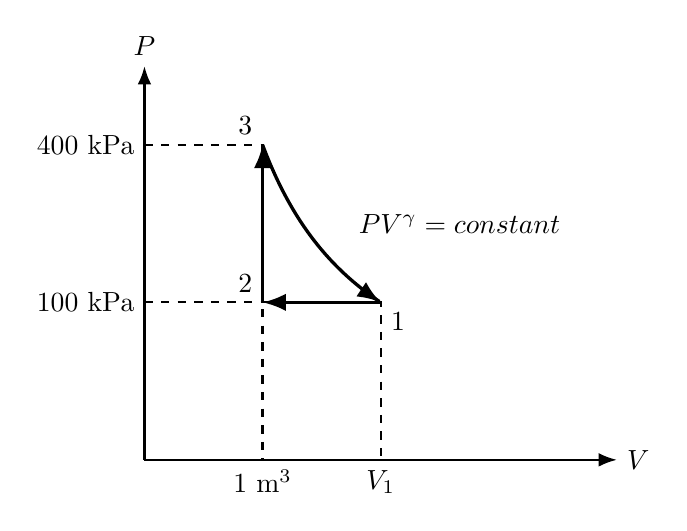
\begin{tikzpicture}[thick]
    % Axes
    \draw[-{Latex}] (0,0) -- (0,5) node[above] {$P$};
    \draw[-{Latex}] (0,0) -- (6,0) node[right] {$V$};

    % Dashed lines for coordinates
    \draw[dashed] (0,4) node[left] {400 kPa} -| (1.5,0) node[below] {1 m$^3$};
    \draw[dashed] (0,2) node[left] {100 kPa} -| (3,0) node[below] {$V_1$};

    % Points and labels
    \node at (1.5,4) [above left] {3};
    \node at (1.5,2) [above left] {2};
    \node at (3,2) [below right] {1};

    % Line segments and hyperbolic curve
    \draw[very thick, -{Latex}] (1.5,2) -- (1.5,4); % Vertical line from 2 to 3
    \draw[very thick, -{Latex}] (3,2) -- (1.5,2); % Horizontal line from 1 to 2

    % Hyperbolic curve from 3 to 1
    \draw[very thick, -{Latex}] plot[domain=1.5:3, samples=100] (\x, {6/\x});
    \node at (4,3) {$PV^\gamma = \text{constant}$}; % Label positioned near the curve

\end{tikzpicture}
\end{center}
\begin{enumerate}
	
\item \usetikzlibrary{decorations.markings, arrows, arrows.meta}


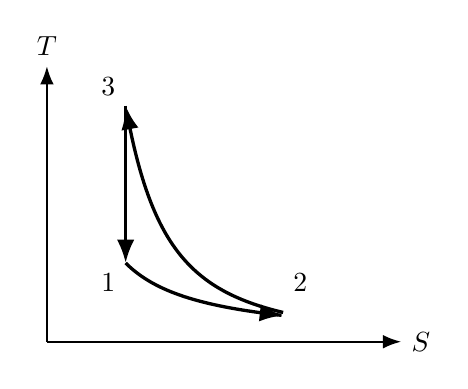
\begin{tikzpicture}[thick]
    % Shortened Axes
    \draw[-{Latex}] (0,0) -- (0,3.5) node[above] {$T$};
    \draw[-{Latex}] (0,0) -- (4.5,0) node[right] {$S$};

    % Points and labels
    \node at (1,3) [above left] {3};
    \node at (1,1) [below left] {1};
    \node at (3,1) [below right] {2};

    
   \draw[very thick, -{Latex}] (1,3) -- (1,1); 

    % Hyperbolic curve from 3 to 1
    \draw[very thick, -{Latex}] plot[domain=1:3, samples=100] (\x, {1/\x});
    \draw[very thick, -{Latex}] plot[domain=3:1, samples=100] (\x, {3/\x^(1.9)});
\end{tikzpicture}
 \item	\usetikzlibrary{decorations.markings, arrows, arrows.meta}


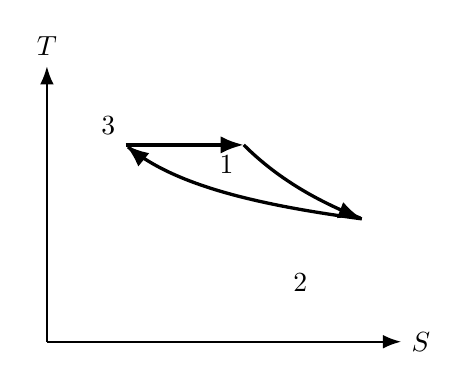
\begin{tikzpicture}[thick]
    % Shortened Axes
    \draw[-{Latex}] (0,0) -- (0,3.5) node[above] {$T$};
    \draw[-{Latex}] (0,0) -- (4.5,0) node[right] {$S$};

    % Points and labels
    \node at (1,2.5) [above left] {3};
    \node at (2.5,2.5) [below left] {1};
    \node at (3,1) [below right] {2};

    % Straight line from point 3 to point 1
    \draw[very thick, -{Latex}] (1,2.5) -- (2.5,2.5);

    % Hyperbolic curve from 3 to 1
    \draw[very thick, -{Latex}] plot[domain=2.5:4, samples=100] (\x, {6.25/\x});

    % Additional hyperbolic curve with specified domain
    \draw[very thick, -{Latex}] plot[domain=4:1, samples=100] (\x, {2.5/\x^0.34});
\end{tikzpicture}
\item \usetikzlibrary{decorations.markings, arrows.meta}


\begin{tikzpicture}[thick, scale=0.75, every node/.style={scale=0.75}]
    % Arrows and lines
    \draw [line width=0.5pt, ->, >=Stealth] (7.5,9.75) -- (11.25,9.75);
    \draw [line width=1.5pt, ->, >=Stealth] (7.5,9.75) -- (7.5,13.75);
    \draw [line width=1pt, ->, >=Stealth] (10.5,13.25) -- (10.5,12.5);
    \draw [line width=1pt, short] (10.5,12.5) -- (10.5,11.75);
    \draw [line width=1pt, ->, >=Stealth] (10.5,11.75) .. controls (10,11) and (10.25,11) .. (9.5,10.75);
    \draw [line width=1pt, short] (9.5,10.75) -- (8.75,10.5);
    \draw [line width=1pt, ->, >=Stealth] (8.75,10.5) .. controls (9.5,11.5) and (9.75,11.5) .. (10,12.25);
    \draw [line width=1pt, short] (10,12.25) -- (10.5,13.25);

    % Node Labels
    \node [font=\small] at (10.75,13.5) {3};
    \node [font=\small] at (10.75,11.75) {1};
    \node [font=\small] at (8.5,10.25) {2};
    \node [font=\normalsize] at (7.5,14.25) {T};
    \node [font=\normalsize] at (11.5,9.75) {S};
\end{tikzpicture}
\item  \usetikzlibrary{decorations.markings, arrows.meta}



\begin{tikzpicture}[thick, scale=0.75, every node/.style={scale=0.75}]
    % Arrows and lines
    \draw [->, >=Stealth] (7.5,13.5) -- (7.5,16.75);
    \draw [->, >=Stealth] (7.5,13.5) -- (10.75,13.5);
    \draw [line width=0.9pt, ->, >=Stealth] (9.5,16.25) -- (10,16.25);
    \draw [line width=0.9pt, short] (10,16.25) -- (10.25,16.25);
    \draw [line width=0.9pt, ->, >=Stealth] (10.25,16.25) .. controls (10.5,15.25) and (10,15) .. (9.75,14.75) ;
    \draw [line width=1pt, short] (9.75,14.75) .. controls (9.25,14.5) and (9.25,14.25) .. (8.75,14.25);
    \draw [line width=0.9pt, ->, >=Stealth] (8.75,14.25) .. controls (9.5,15) and (9.5,15.25) .. (9.5,15.75) ;
    \draw [line width=0.9pt, short] (9.5,15.75) -- (9.5,16.25);

    % Node Labels
    \node [font=\small] at (10.5,16.5) {1};
    \node [font=\small] at (8.5,14) {2};
    \node [font=\small] at (9.25,16.5) {3};
    \node [font=\normalsize] at (7.5,17.25) {T};
    \node [font=\normalsize] at (11,13.5) {S};
\end{tikzpicture}
\end{enumerate}
\item If the specific heats of the working fluid are constant and the value of specific heat ratio $\gamma$ is 1.4, the thermal efficiency (\%) of the cycle is
\begin{enumerate}
	\item 21 
	\item 40.9 
	\item 42.6 
	\item 59.7
\end{enumerate}
\textbf{Linked Answer Questions: Q.76 to Q.85}

\subsection{Statement for Linked Answer Questions 76 \& 77:}

Consider a steady incompressible flow through a channel as shown below.
\begin{center}
\usetikzlibrary{decorations.markings, arrows.meta}

\begin{tikzpicture}[thick, scale=0.75, every node/.style={scale=0.75}]
    % Horizontal lines
    \draw [line width=0.2pt] (3,10.5) to[short] (9.75,10.5);
    \draw [line width=0.2pt] (3,7.75) to[short] (10,7.75);
    \draw [line width=0.2pt] (3,10.5) to[short] (3,7.75);
    \draw [line width=0.2pt] (2.25,10.5) to[short] (2.25,7.75);
    
    % Arrows
    \draw [line width=0.2pt, ->, >=Stealth] (2.25,10.5) -- (3,10.5);
    \draw [line width=0.2pt, ->, >=Stealth] (2.25,10) -- (3,10);
    \draw [line width=0.2pt, ->, >=Stealth] (2.25,9.5) -- (3,9.5);
    \draw [line width=0.2pt, ->, >=Stealth] (2.25,9) -- (3,9);
    \draw [line width=0.2pt, ->, >=Stealth] (2.25,8.25) -- (3,8.25);
    \draw [line width=0.2pt, ->, >=Stealth] (2.25,7.75) -- (3,7.75);
    
    % Vertical lines
    \draw [line width=0.2pt] (7,10.5) to[short] (7,7.75);
    \draw [line width=0.2pt] (8,10.5) to[short] (8,7.75);
    
    % Dashed lines
    \draw [line width=0.2pt, ->, >=Stealth, dashed] (7,10) -- (8,10);
    \draw [line width=0.2pt, short] (7,10.5) -- (8,10);
    \draw [line width=0.2pt, ->, >=Stealth, dashed] (7,8.25) -- (8,8.25);
    \draw [line width=0.2pt, short] (8,8.25) -- (7,7.75);
    
    % Additional lines
    \draw [line width=0.2pt] (8,10) to[short] (8.75,10);
    \draw [line width=0.2pt] (8,8.25) to[short] (8.75,8.25);
    
    % Double arrows
    \draw [line width=0.2pt, <->, >=Stealth] (8.75,10.5) -- (8.75,10);
    \draw [line width=0.2pt, <->, >=Stealth] (8.75,8.25) -- (8.75,7.75);
    \draw [line width=0.2pt, <->, >=Stealth] (9.75,10.5) -- (9.75,7.75);
    
    % Output arrow
    \draw [->, >=Stealth] (10,7.75) -- (11.25,7.75);
    
    % Node Labels
    \node [font=\LARGE] at (11.25,7.25) {x};
    \node [font=\normalsize] at (9.5,9.25) {H};
    \node [font=\normalsize] at (9,10.25) {$\delta$};
    \node [font=\normalsize] at (9,8) {$\delta$};
    
    % Lines connecting V_m and A/B
    \draw [->, >=Stealth] (7,8.75) -- (8,8.75);
    \draw [line width=0.2pt, ->, >=Stealth] (7,9.25) -- (8,9.25);
    \node [font=\normalsize] at (7.5,9.5) {$V_m$};
    \node [font=\normalsize] at (2.5,9.75) {$u_o$};
    
    % More arrows and node labels
    \draw [line width=0.2pt, ->, >=Stealth] (7,9.75) -- (8,9.75);
    \draw [line width=0.2pt, ->, >=Stealth] (3,10.5) -- (3,11.25);
    \node [font=\large] at (3,7.5) {A};
    \node [font=\large] at (8,7.5) {B};
    
    % Dashed connecting lines
    \draw [line width=0.2pt, dashed] (3,7.75) -- (3.25,8);
    \draw [line width=0.2pt, dashed] (3.25,8) -- (3.5,8);
    \draw [line width=0.2pt, dashed] (3.5,8) -- (7,8.25);
    \draw [line width=0.2pt, dashed] (3,10.5) -- (7,10);
    
    % Label for Y
    \node [font=\large] at (2.5,11) {Y};

\end{tikzpicture}
\end{center}
The velocity profile is uniform with a value of $u_0$ at the inlet section A. The velocity profile at section B downstream is
\[
u = 
\begin{cases} 
      V_m \frac{y}{\delta} & 0 \leq y \leq \delta \\
      V_m & \delta \leq y \leq H - \delta \\
      V_m \frac{H - y}{\delta} & H - \delta \leq y \leq H 
   \end{cases}
\]

\item The ratio $V_m / u_0$ is

\begin{enumerate}
	\item $\frac{1}{1 - 2\brak{\delta / H}}$
    \item 1
    \item $\frac{1}{1 - \brak{\delta / H}}$
    \item $\frac{1}{1 + \brak{\delta / H}}$
\end{enumerate}

\item The ratio $\frac{p_A - p_B}{\frac{1}{2} \rho u_0^2}$ (where $p_A$ and $p_B$ are the pressures at section A and B, respectively, and $\rho$ is the density of the fluid) is

\begin{enumerate}
	\item $\frac{1}{\brak{ 1 - \brak{\delta / H}}^2} - 1$
	\item $\frac{1}{\sbrak{ 1 - \brak{\delta / H} }^2}$

	\item $\frac{1}{\brak{ 1 - 2\brak{\delta / H}}^2} - 1$
	\item $\frac{1}{1 + \brak{\delta / H}} $
\end{enumerate}
\subsection{Statement for Linked Answer Questions 78 \& 79:}

Consider steady one-dimensional heat flow in a plate of 20 mm thickness with a uniform heat generation of 80 MW/m$^3$. The left and right faces are kept at constant temperatures of 160$^\circ$C and 120$^\circ$C respectively. The plate has a constant thermal conductivity of 200 W/mK.

\item The location of maximum temperature within the plate from its left face is
    \begin{enumerate}
        \item 15 mm
        \item 10 mm
        \item 5 mm
        \item 0 mm
    \end{enumerate}
    
    \item The maximum temperature within the plate in $^\circ$C is
    \begin{enumerate}
        \item 160
        \item 165
        \item 200
        \item 250
    \end{enumerate}

\subsection{Statement for Linked Answer Questions 80 \& 81:}

A machine frame shown in the figure below is subjected to a horizontal force of 600 N parallel to $z$-direction.
\begin{center}

\usetikzlibrary{decorations.markings, arrows.meta}


\begin{tikzpicture}[thick, scale=0.75, every node/.style={scale=0.75}]
    % Short lines and connections
    \draw [line width=0.2pt, short] (5.5,9.75) -- (3.25,7.75);
    \draw [line width=0.2pt, short] (5.5,9.75) -- (7,8.25);
    \draw [line width=0.2pt, short] (7,8.25) -- (4.75,6.25);
    \draw [line width=0.2pt, short] (3.25,7.75) -- (4.75,6.25);
    \draw [line width=0.2pt, short] (4.75,6.25) -- (4.75,6);
    \draw [line width=0.2pt, short] (3.25,7.75) -- (3.25,7.5);
    \draw [line width=0.2pt, short] (7,8.25) -- (7,8);
    \draw [line width=0.2pt, short] (7,8) -- (4.75,6);
    \draw [line width=0.2pt, short] (3.25,7.5) -- (4.75,6);
    \draw [line width=0.2pt, short] (4.25,8.75) -- (6.5,6.5);
    \draw [line width=0.2pt, short] (5,8) -- (3.75,6.75);
    
    % Ellipses
    \draw [line width=0.2pt] (1.5,5.5) ellipse (0cm and 0.25cm);
    \draw [line width=0.2pt, short] (4.75,8) -- (4.75,12);
    
    % Sinusoidal function
    \draw[domain=4.75:5,samples=100,smooth, line width=0.2pt] plot (\x,{1*sin(1*\x r -4.75 r ) +12});
    
    % Additional short lines
    \draw [line width=0.2pt, short] (5,12.25) -- (5.25,12.25);
    \draw [line width=0.2pt, short] (5.25,12.25) -- (11.25,8.25);
    \draw [line width=0.2pt, short] (5.25,8) -- (5.25,11.5);
    \draw [line width=0.2pt, short] (5.25,11.5) -- (11,7.75);
    
    % More ellipses
    \draw [line width=0.2pt] (11,8) ellipse (0.25cm and 0.25cm);
    \draw [line width=0.2pt] (5,8) ellipse (0.25cm and 0.25cm);
    
    % Dashed lines
    \draw [line width=0.2pt, dashed] (5,8.25) -- (5,11.75);
    \draw [line width=0.2pt, dashed] (5,11.75) -- (5.25,11.75);
    \draw [line width=0.2pt, dashed] (5.25,11.75) -- (10.75,8.25);
    \draw [line width=0.2pt, dashed] (5,11.75) -- (5,13);
    
    % More short lines
    \draw [line width=0.2pt, short] (11,8) -- (11,9.5);
    
    % Double-headed arrow
    \draw [line width=0.2pt, <->, >=Stealth] (5,12.75) -- (11,9) node[pos=0.5, fill=white]{500 mm};
    \node [font=\small] at (4.75,12.5) {y};
    
    % More connections
    \draw [line width=0.2pt, short] (4.5,12.25) -- (4,12.5);
    \draw [line width=0.2pt, <->, >=Stealth] (4,12.5) -- (4,8.75) node[pos=0.5, fill=white]{300 mm};
    \draw [line width=0.2pt, ->, >=Stealth] (4.25,10.5) -- (4.75,10);
    \draw [line width=0.2pt, ->, >=Stealth] (5.75,10) -- (5.25,10.25);
    \draw [line width=0.2pt, ->, >=Stealth, dashed] (10,7.5) -- (11,8);
    
    % Node labels
    \node [font=\small] at (6,10.25) {$\Phi$ 30 mm};
    \node [font=\small] at (5,8) {P};
    \node [font=\small] at (3.75,6.75) {Z};
    \node [font=\small] at (6.5,6.75) {X};
    \node [font=\small] at (10.25,7.5) {600 N};
    
    % Additional short lines
    \draw [line width=0.2pt, short] (3.5,7.5) -- (3.25,7.75);
    \draw [line width=0.2pt, short] (5,6.5) -- (5,6.25);
    \draw [line width=0.2pt, short] (5.25,6.75) -- (5.25,6.5);
    \draw [line width=0.2pt, short] (5.5,7) -- (5.5,6.75);
    \draw [line width=0.2pt, short] (6.75,8) -- (6.75,7.75);
    \draw [line width=0.2pt, short] (6.5,7.75) -- (6.5,7.5);
    \draw [line width=0.2pt, short] (6.25,7.5) -- (6.25,7.25);
    \draw [line width=0.2pt, short] (6,7.5) -- (6,7.25);
    \draw [line width=0.2pt, short] (4.5,6.5) -- (4.5,6.25);
    \draw [line width=0.2pt, short] (4.25,6.75) -- (4.25,6.5);
    \draw [line width=0.2pt, short] (4,7) -- (4,6.75);
    \draw [line width=0.2pt, short] (3.75,7.25) -- (3.75,7);
    \draw [line width=0.2pt, short] (3.5,7.5) -- (3.5,7.25);
    \draw [line width=0.2pt, short] (3.25,7.75) -- (3.25,7.5);

\end{tikzpicture}
\end{center}
    \item The normal and shear stresses in MPa at point $P$ are respectively
    \begin{enumerate}
        \item 67.9 and 56.6
        \item 56.6 and 67.9
        \item 67.9 and 0.0
        \item 0.0 and 56.6
    \end{enumerate}

    \item The maximum principal stress in MPa and the orientation of the corresponding principal plane in degrees are respectively
    \begin{enumerate}
        \item $-32.0$ and $-29.52$
        \item 100.0 and 60.48
        \item $-32.0$ and 60.48
        \item 100.0 and $-29.52$
    \end{enumerate}

\subsection{Statement for Linked Answer Questions 82 \& 83:}

A quick return mechanism is shown below. The crank OS is driven at 2 rev/s in counter-clockwise direction.
\begin{center}
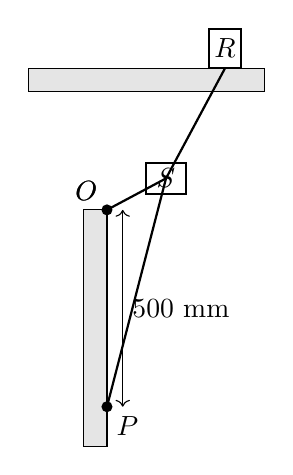
\begin{tikzpicture}
    % Draw the vertical wall
    \draw[fill=gray!20] (-0.3,-3) rectangle (0,0);

    % Draw the horizontal support for block R
    \draw[fill=gray!20] (-1,1.5) rectangle (2,1.8);

    % Draw point P
    \fill (0,-2.5) circle (2pt) node[below right] {$P$};

    % Draw point O (pivot)
    \fill (0,0) circle (2pt) node[above left] {$O$};

    % Draw the vertical dimension line for 500 mm
    \draw[<->] (0.2,0) -- (0.2,-2.5) node[midway, right] {500 mm};

    % Draw block R as a rectangle above
    \draw[thick] (1.3,1.8) rectangle (1.7,2.3) node[midway] {$R$};

    % Draw block S as a rectangle
    \draw[thick] (0.5,0.2) rectangle (1.0,0.6) node[midway]{ $S$ };

    % Draw the connections between points without passing through blocks
    \draw[thick] (1.5,1.8) -- (0.75,0.4); % Connecting R to S
    \draw[thick] (0.75,0.4) -- (0,0);     % Connecting S to O
    \draw[thick] (0,0) -- (0,-2.5);       % Connecting O to P
    \draw[thick] (0,-2.5) -- (0.75,0.4);  % Connecting P to S directly

    % Label point O
    \node[above left] at (0,0) {$O$};
    % Label point S only once, placing it effectively
    \node[above right] at (0.75,0.4) { };

\end{tikzpicture}
\end{center}
    \item If the quick return ratio is 1:2, then the length of the crank in mm is
    \begin{enumerate}
        \item 250
        \item 250$\sqrt{3}$
        \item 500
        \item 500$\sqrt{3}$
    \end{enumerate}
    
    \item The angular speed of PQ in rev/s when the block R attains maximum speed during forward stroke (stroke with slower speed) is
    \begin{enumerate}
	\item $\frac{1}{3}$
	\item $\frac{2}{3}$
        \item 2
        \item 3
    \end{enumerate}

\subsection{Statement for Linked Answer Questions 84 \& 85:}

A low carbon steel bar of 147 mm diameter with a length of 630 mm is being turned with uncoated carbide insert. The observed tool lives are 24 min and 12 min for cutting velocities of 90 m/min and 120 m/min respectively. The feed and depth of cut are 0.2 mm/rev and 2 mm respectively. Use the unmachined diameter to calculate the cutting velocity.

    \item When tool life is 20 min, the cutting velocity in m/min is
    \begin{enumerate}
        \item 87
        \item 97
        \item 107
        \item 114
    \end{enumerate}
    
    \item Neglect over-travel or approach of the tool. When tool life is 20 min, the machining time in min for a single pass is
    \begin{enumerate}
        \item 5
        \item 10
        \item 15
        \item 20
    \end{enumerate}
